\documentclass[12pt]{article} %set font size and document type
\usepackage{graphicx} % Required for inserting images
\usepackage[useregional]{datetime2} %allow use of \today
\usepackage[margin=1in]{geometry} % set margins
\usepackage{setspace} % allow setting of double and single spacing
\usepackage{hyperref} % creates clickable table of contents
\usepackage{adjustbox} % allows us to rotate images, tables, etc.

% \usepackage{xcolor}
\usepackage{color, colortbl}

\usepackage{listings}
\newcommand{\lsin}[1]{\lstinline[columns=fullflexible,keepspaces=true,language=Java,basicstyle=\footnotesize\ttfamily]{#1}}

\lstdefinelanguage{Java}{
  columns=fullflexible,keepspaces=true,basicstyle=\scriptsize\ttfamily,
%  basicstyle=\scriptsize\sffamily,
  numbers=left,
  xleftmargin=5.0ex,
  escapechar=@,
  sensitive=true,
  otherkeywords={},
  morekeywords=[1]{int,while,if,public,static,else,return,new,for,return,void},
  keywordstyle={[1]\bfseries\color{blue}},
  numberstyle=\tiny\color{black},
  rulecolor=\color{black},
}

% set up header and footer
\usepackage{titleps,kantlipsum}
\newpagestyle{mypage}{%
  \headrule
  \sethead{\MakeUppercase{\thesection\quad \sectiontitle}}{}{\thesubsection\quad \subsectiontitle}
  \setfoot{}{}{\em{p. \thepage}}
}
\settitlemarks{section,subsection}
\pagestyle{mypage}

% set up title information 
% Students replace project title and their names here
\title{War Card Game
\\
CS482 Software Engineering}
\author{Ayoposi Olu-Bamisaye, Jonathan Ramos, Brett Bonner\\
Client: Dr. Eric Cui}
\date{\today}

\begin{document}

\maketitle

\pagebreak


\section{Design}

\subsection{Architecture}
We are planning on implementing a Model View Controller (MVC) architecture type for our game. It will be able to handle our in-game logic and how the user interacts with the game itself.
The Model typically will represent the game logic, deck and cards. The View will be responsible for representing the current state of the game to the user. Examples of this are displaying the players stats, profile and friends, having the ability to view output of cards/deck and showing tables in the lobby. We will be using a graphical feature to show this in our project. The Controller will handle user input for various commands like starting the game, ending the game, placing cards, party privacy and updating the players profile settings.

\subsection{Technologies}
Since we are developing a web-based version of the card game ``War", we have decided to use modern web technologies to ensure we have a responsive and scale-able application. Our front end will consist of common technologies used for web development, HTML, CSS, and Javascript. HTML will provide the basic structure of the web page, and CSS will allow us to style the page according to the theme specified by Cosmic Radiance. Javascript will handle game logic on the client side. Our front-end framework will be React.js as this will facilitate with updating the game-state without refreshing the page. React will also help with creating reusable components such as the cards themselves. 

Our back end will need to handle the game logic, player data, and real-time communication. Node.js will allow us to handle game logic outside of the browser. This will allow us the necessary means of handling requests such as determining winners. We will use a library Socket.io to handle real-time communication between multiple clients. 

To store our user data, game history, and player stats we will need persistent storage. We have chosen Firebase as our persistent storage due to its ease of use with real-time updates. It will also allow us to have a more flexible schema as SQL databases require relations among the tables created. Firebase also includes built-in authentication, supporting Google and Facebook sign in, as well as traditional email and password. Overall, Firebase supports our needs of real-time updates, scalability, security, and rapid development. 

\subsection{Persistent Storage}
Our database is composed of three main firebase components, Authentication, Firestore, and Storage. Each of these components is responsible for storing different types of information for each user. The authentication component is responsible for storing user login information, in our application this is the email and password of every user. Importantly, the Authentication component hashes passwords with a built-in function which improves security for our users. The storage component is responsible for storing the profile images of every user. The profile picture uploaded by the user is saved to the storage component under `avatars/user.uid' in which the current user's id is used as the filename. The majority of our user's data will be saved in the Firestore component. The data will be organized as JSON documents which are then organized into collections. The user's information such as, username, friends, stats, and profile picture URL will be saved into a document appropriately titled as the `user.uid'. Each user will require their own document, and all user documents will be stored in the `users' collection. This structure is flexible, making it scale-able which is important for an online multiplayer game. Our NoSQL design ensures that we can continue adding more collections and documents as needed without restructuring the entire database.

\subsection{Coding Standards}
Our database naming scheme will consist of singular, lowercase names for collections (user, leaderboard). Each attribute within documents will use camelCase (userName, gameStats, gameID). Variables and functions in JavaScript should also be written in camelCase. 

We will format our code using two spaces for indentation. Brackets should be used on the same line for functions and other control statements. Inline commenting should be used only to explain complex logic. Multi line comments should be used to describe functions and classes. Additionally, all functions should be properly documented with a multi-line comment describing the purpose, parameters, and return value. 

Testing standards will consist of test-driven development. We will ensure proper functionality by ensuring that all code commits pass necessary code tests before merging. Code tests should handle correctness, edge cases, and performance. 

\section{UML Diagram}
\begin{figure}
    \centering
    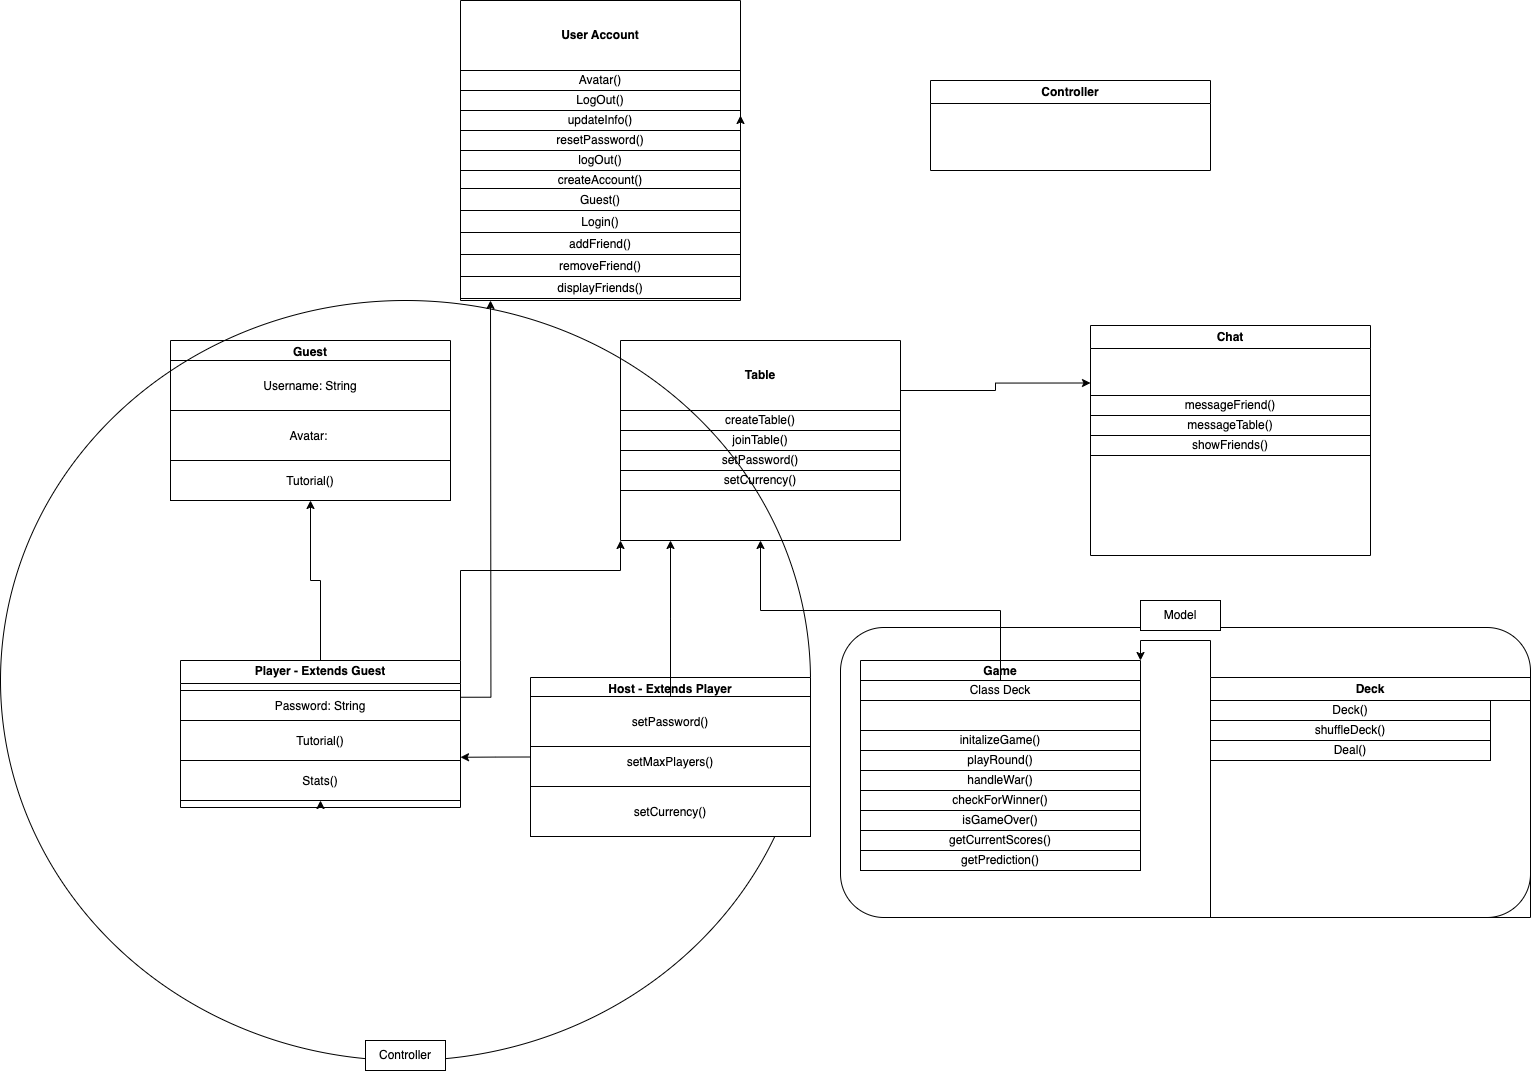
\includegraphics[width=1\linewidth]{figures/WarUML.png}
    \caption{UML diagram outlining the war card game for Cosmic Radiance}
    \label{fig:enter-label}
\end{figure}

The system features a Host class that extends the player class, granting the host control over the table, including decisions on who can join. Additionally, a Game class manages the gameplay mechanics, ensuring that the rules of the game are followed. The User Account class manages all of the information of the User, from their password to avatar, to their friends. Lastly, a table class is made to allow users to join the table or create their own table.

\section {UI Mockups}
\begin{figure}
    \centering
    \includegraphics[width=1\linewidth]{figures/Welcome Page UI.png}
    \caption{The UI design for Cosmic Radiance web app's welcome screen features a space-themed layout with royal blue tones.}
    \label{fig:enter-label}
\end{figure}

\begin{figure}
    \centering
    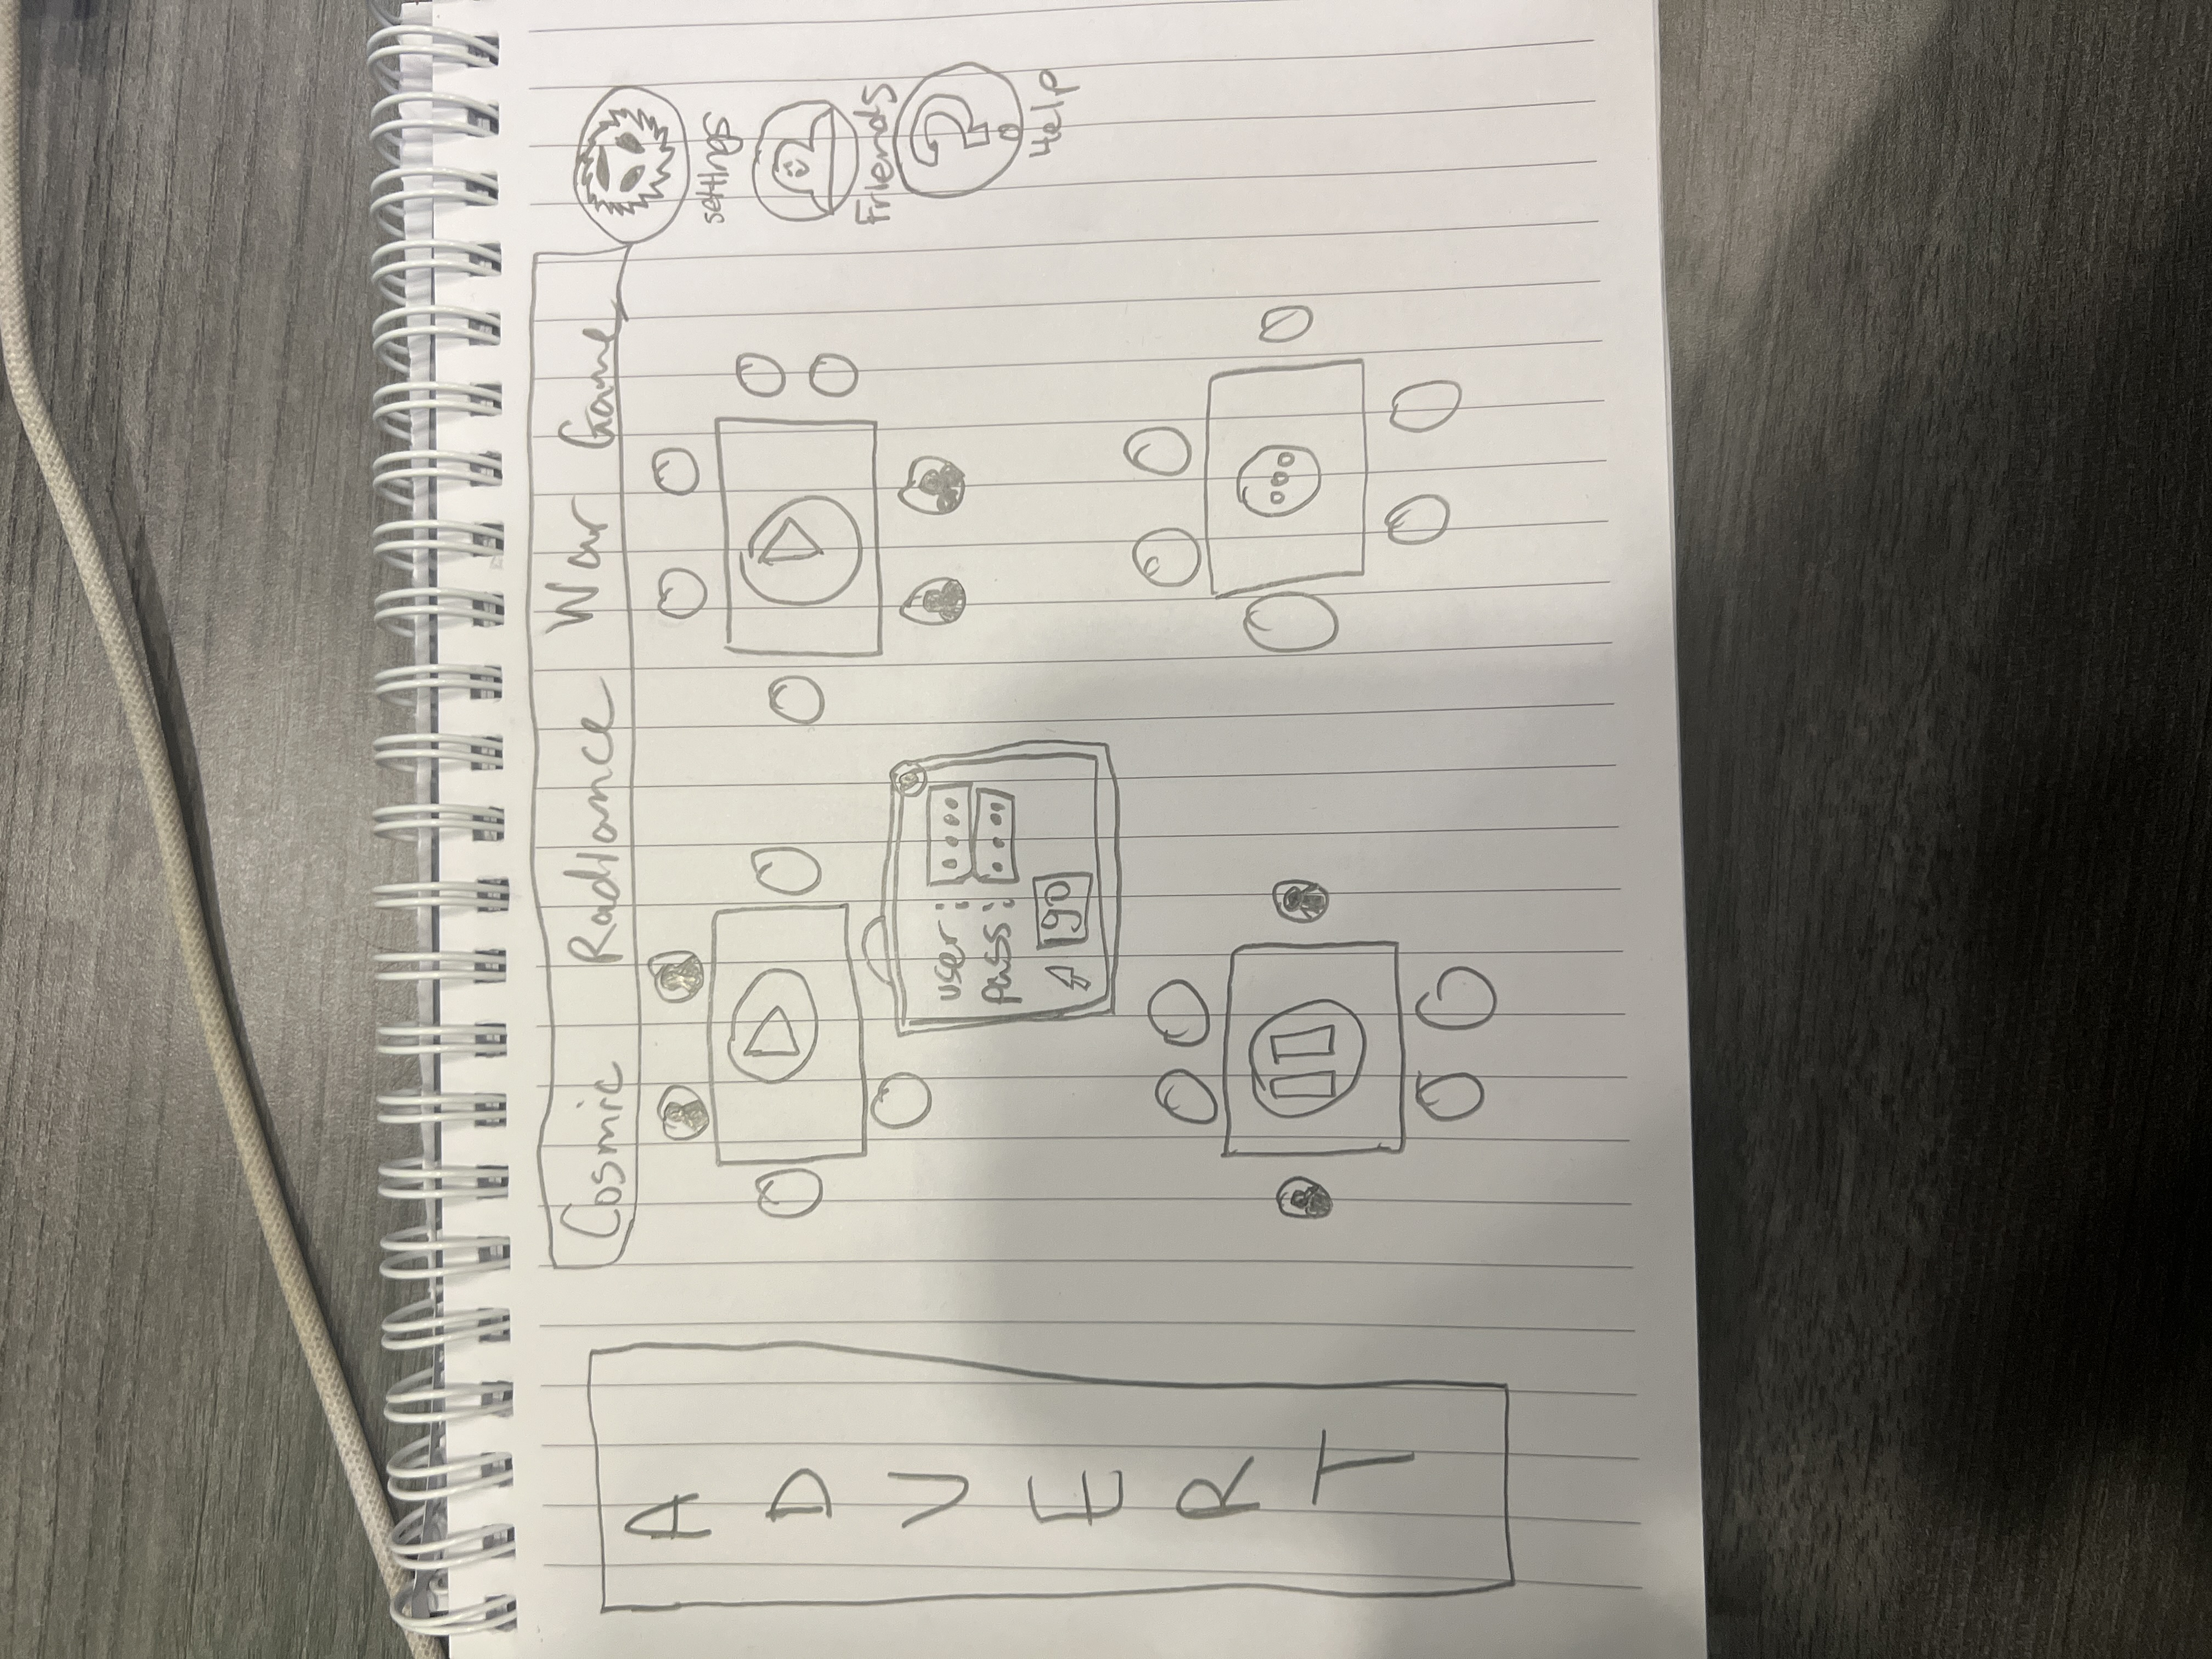
\includegraphics[width=1\linewidth]{figures/Lobby UI.jpeg}
    \caption{Lobby UI.}
    \label{fig:enter-label}
\end{figure}

\begin{figure}
    \centering
    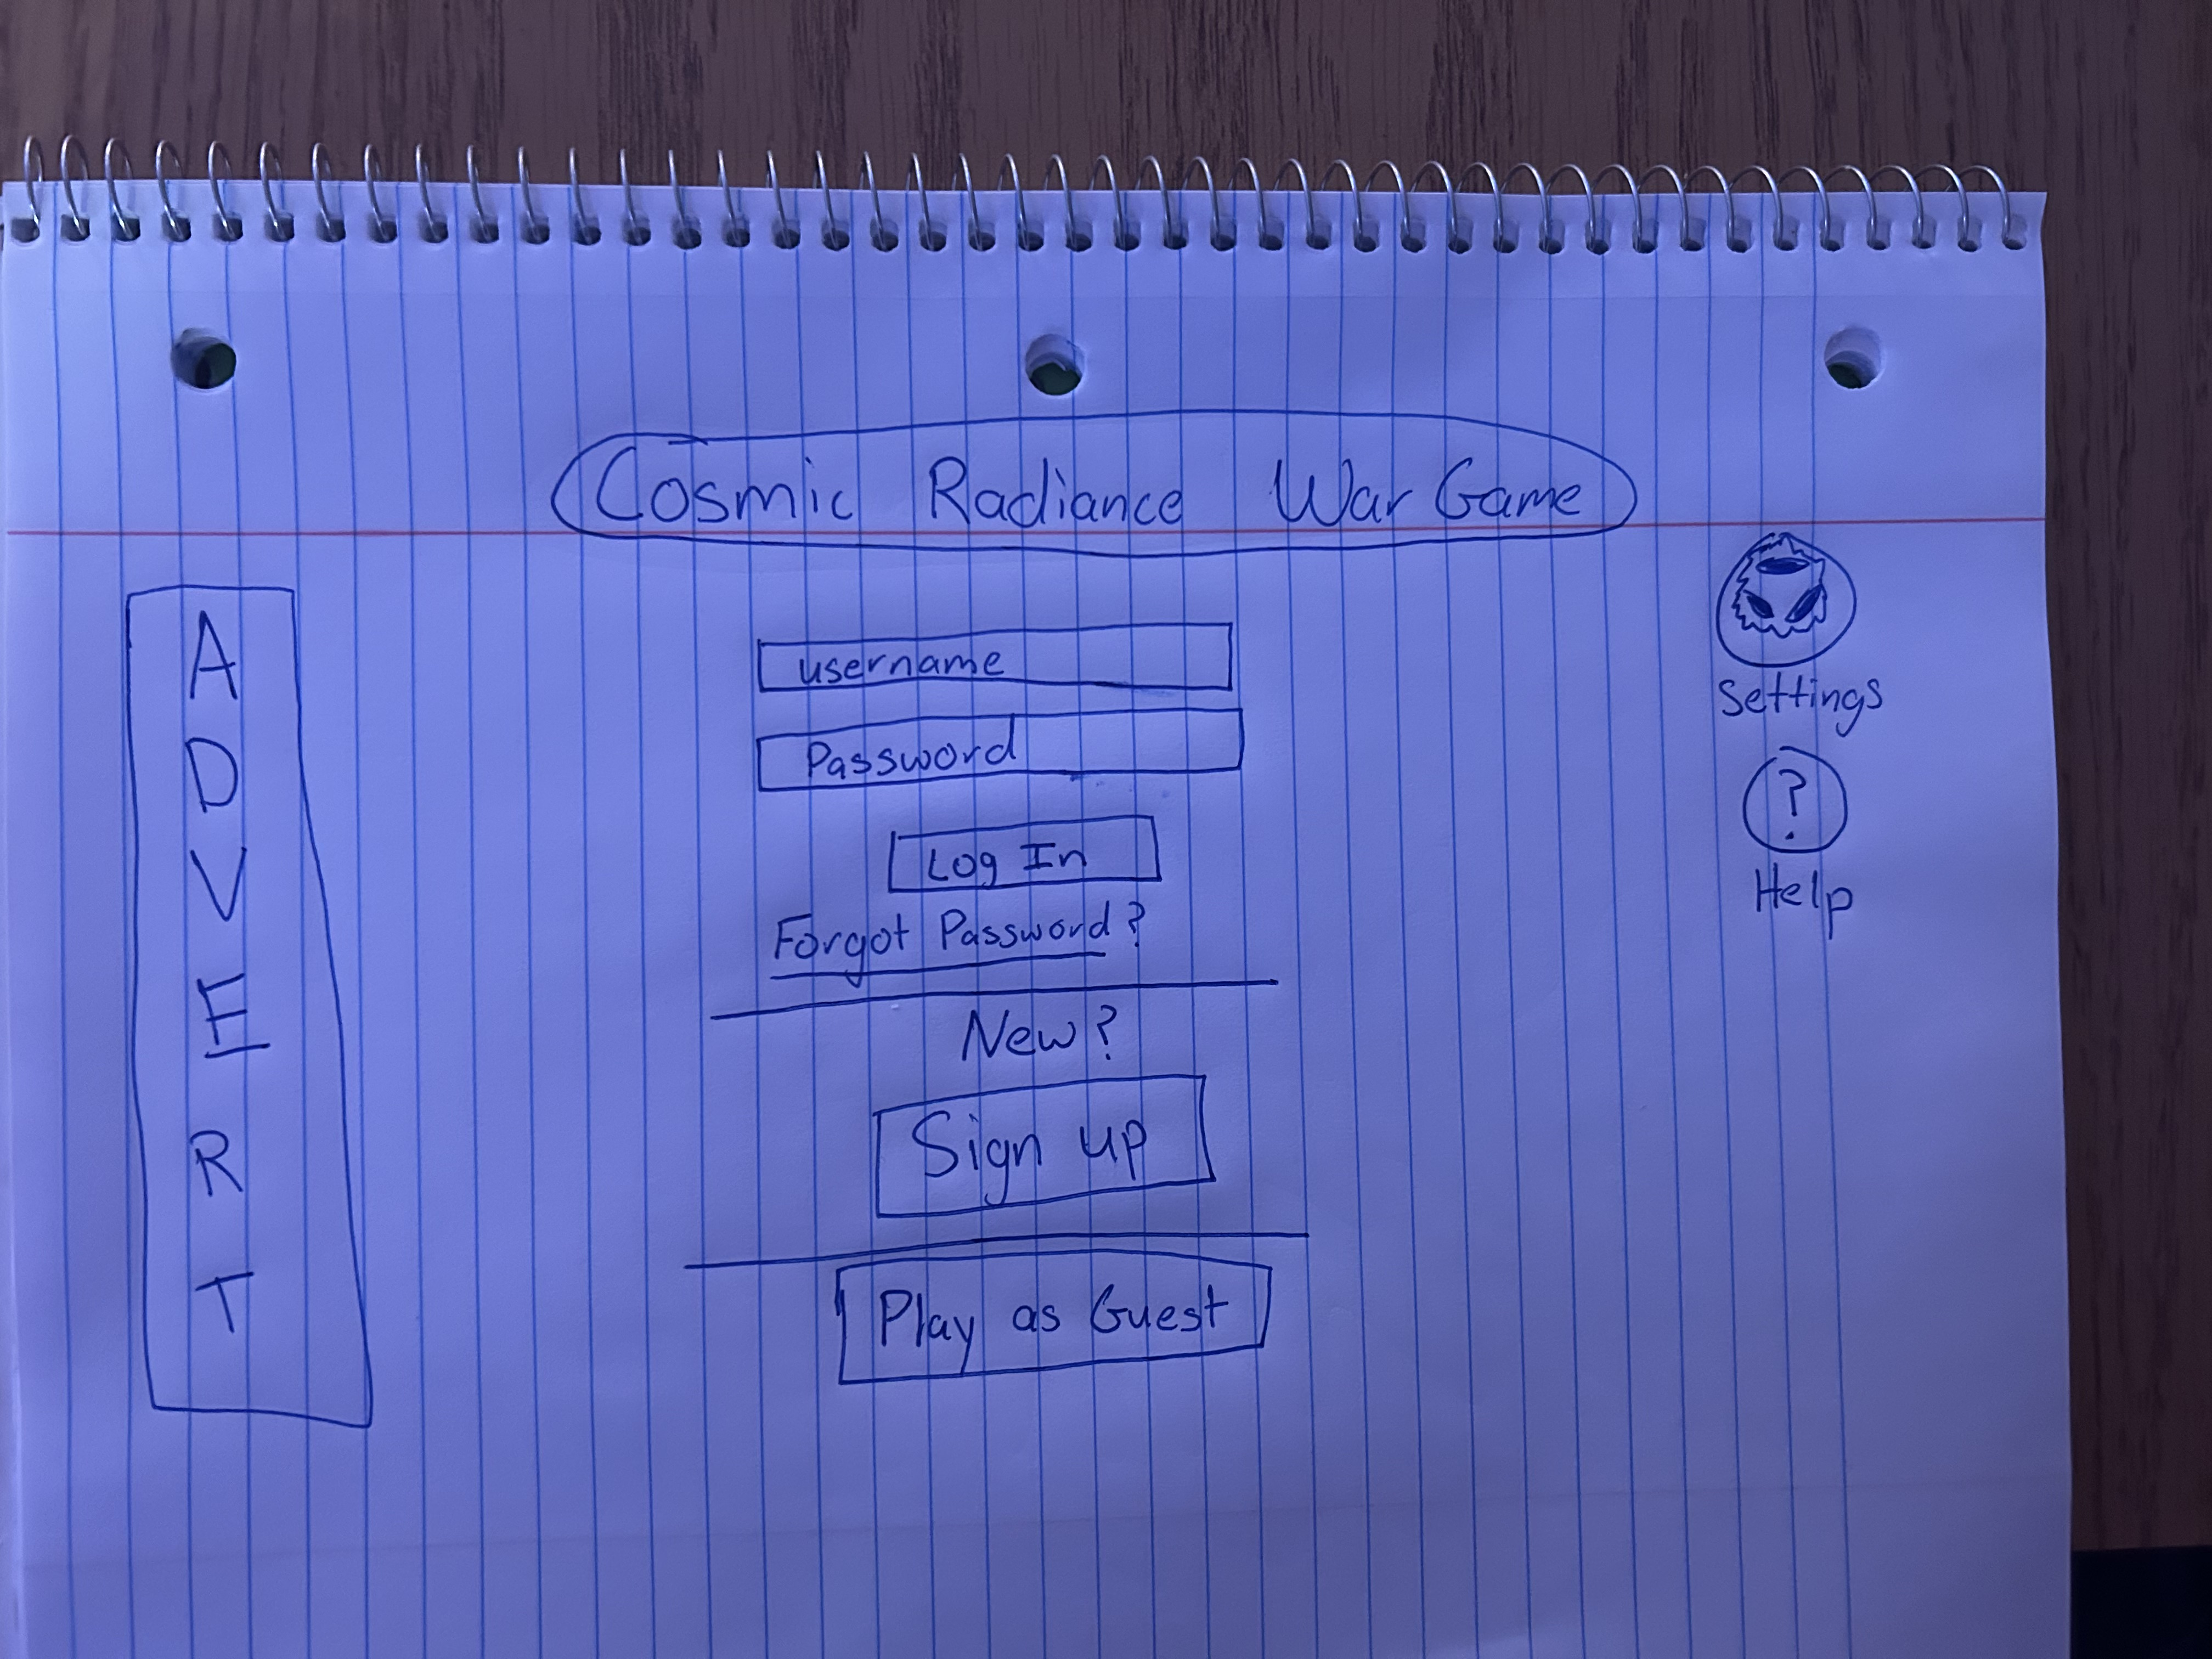
\includegraphics[width=1\linewidth]{figures/Login UI.jpeg}
    \caption{Login Screen for Cosmic Radiance War Game.}
    \label{fig:enter-label}
\end{figure}


\pagebreak

\section {Sprint 1}
\subsection {Testing}
\begin{figure} [h]
    \centering
    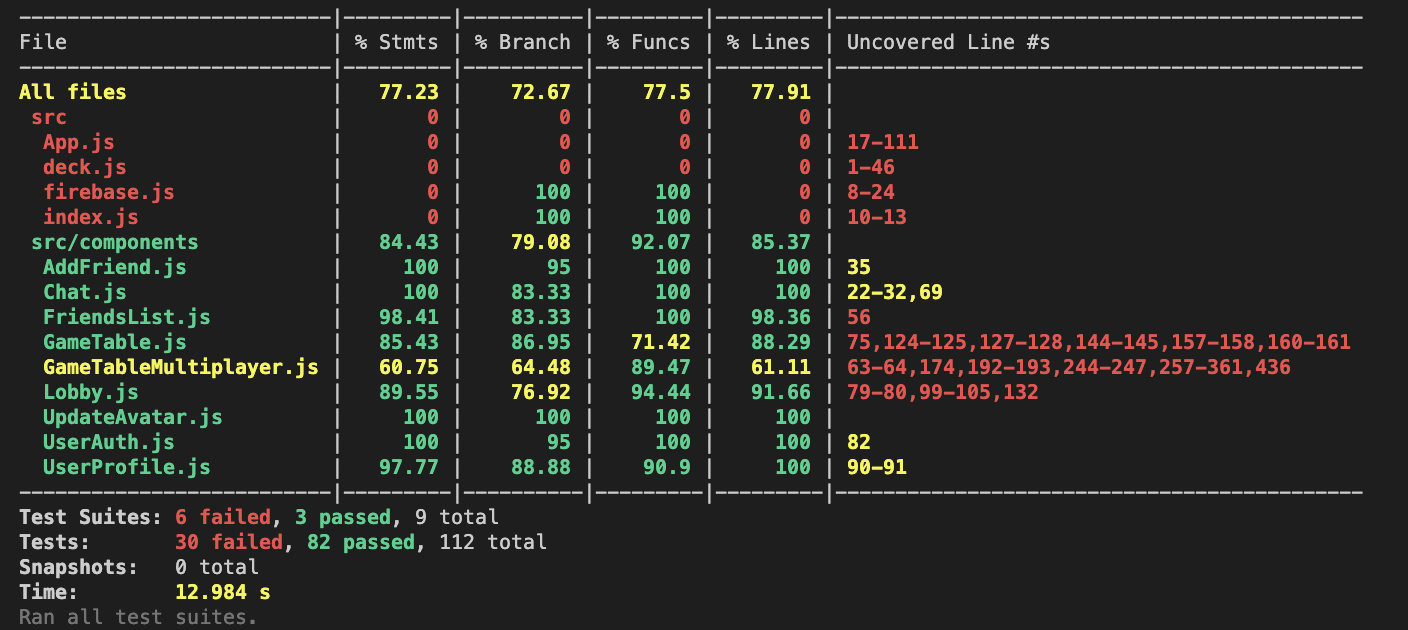
\includegraphics[width=1\linewidth]{figures/Testing.png}
    \caption{Testing Output}
    \label{fig:enter-label}
\end{figure}

    We chose Jest as a testing framework. We attempted to do unit testing for branch and statement coverage, however, we struggled with connecting jest with our react components. We managed to get some of our code tested as shown in firebase.js, AddFriend.js, and UserAuth.js. For our next sprint we plan on solving the issue with testing with a spike to ensure we meet the specified requirements. 

\begin{table}[h]
\centering
No story changes or slices during this sprint.

\caption{Sprint Story Distribution and Point Tracking}
\begin{tabular}{|p{3cm}|p{6cm}|c|c|}
\hline
\textbf{Team Member} & \textbf{Stories Attempted} & \textbf{Points Attempted} & \textbf{Status} \\
\hline
Ayoposi Olu & 
\begin{itemize}
    \item S4: Logout (1 pt)
    \item S5: Password (2 pts)
    \item S6: Update (1 pt)
\end{itemize} & 
4 & 
Completed \\
\hline
Jonathan Ramos & 
\begin{itemize}
    \item S7: Profile Avatar (2 pts)
    \item S8: Add Friend (2 pts)
    \item S9: Remove Friend (2 pts)
    \item S10: Show Friends (1 pt)
\end{itemize}& 
7 & 
Completed \\
\hline
Brett Bonner & 
\begin{itemize}
    \item S1: Create User (2 pts)
    \item S2: Guest Account (1 pt)
    \item S3: Login (1 pt)
\end{itemize} & 
4 & 
Completed \\
\hline
\multicolumn{4}{|c|}{} \\
\hline
\multicolumn{2}{|l|}{\textbf{Total Points Attempted}} & \multicolumn{2}{c|}{15} \\
\hline
\multicolumn{2}{|l|}{\textbf{Total Sprint Points (All Stories)}} & \multicolumn{2}{c|}{62} \\
\hline
\end{tabular}

\vspace{0.5cm}
\begin{center}
\small{Sprint period from 10/17/2024 to 10/24/2024}
\end{center}
\end{table}

\begin{table}[h]
\centering
\caption{Team Velocity and Hours-per-Point Metrics}
\begin{tabular}{|l|c|c|c|}
\hline
\textbf{Team Member} & \textbf{Hours Worked} & \textbf{Story Points} & \textbf{Hours/Point} \\
\hline
Ayoposi Olu & 12 & 4 & 3 \\
\hline
Jonathan Ramos & 20 & 7 & 2.85 \\
\hline
Brett Bonner & 13 & 4 & 3.25 \\
\hline
\multicolumn{4}{|c|}{} \\
\hline
\multicolumn{2}{|l|}{\textbf{Team Totals}} & \textbf{14} & \textbf{2.857} \\
\hline
\end{tabular}

\begin{center}
\small{Sprint Velocity History}
\end{center}
\begin{tabular}{|l|c|c|c|c|}
\hline
\textbf{Sprint} & \textbf{Points Completed} & \textbf{Hours Worked} & \textbf{Hours/Point} & \textbf{Velocity} \\
\hline
Sprint 1 & 14 & 45 & 3 & 14 pts/sprint \\
\hline
\end{tabular}

\vspace{0.5cm}
\begin{center}
\small{Velocity = Points completed per sprint \\
Hours/Point = Total hours worked / Points completed}
\end{center}
\end{table}





\end{document}


